\documentclass[a4paper,12pt]{article}
\usepackage{geometry}
\geometry{left=2cm}
\geometry{right=1.5cm}
\geometry{top=3cm}
\geometry{bottom=3cm}

\usepackage[unicode=true, colorlinks=false, hidelinks]{hyperref}
\usepackage[utf8]{inputenc}
\usepackage[english, russian]{babel}
\usepackage{mathtext}
\usepackage[T2A, TS1]{fontenc}
\usepackage{microtype} % Slightly tweak font spacing for aesthetics
\usepackage{amsthm, amssymb, amsmath, amsfonts, nccmath}
\usepackage{nicefrac}
\usepackage{epstopdf}
\usepackage[export]{adjustbox}
\usepackage{float} % Improved interface for floating objects
\usepackage{graphicx, multicol} % Enhanced support for graphics
\usepackage{pdfrender,xcolor}

\usepackage{mathtools}
\usepackage{titling}
\usepackage{bm}
\usepackage{centernot}
\usepackage[cal=boondoxo,calscaled=.96]{mathalpha}
\usepackage{marvosym, wasysym} % More symbols
\usepackage{rotating} % Rotation tools
\usepackage{censor} % Facilities for controlling restricted text
\usepackage{indentfirst}
\usepackage{svg}

\DeclareMathOperator{\cov}{cov}
\DeclareMathOperator{\med}{med}
\DeclareMathOperator{\sign}{sign}

\usepackage{array}
\newcolumntype{C}[1]{>{\centering\let\newline\\\arraybackslash\hspace{0pt}}m{#1}}

\usepackage{fancyhdr}
\pagestyle{fancy}
\fancyhead{}\renewcommand{\headrulewidth}{0pt}
\fancyfoot[L]{}
\fancyhead{}
\fancyfoot{}
\fancyfoot[R]{\thepage}
\begin{document}
\begin{titlepage}
	\newpage
	
	\begin{center}
		\textrm{\large Санкт-Петербургский политехнический университет \linebreak Петра Великого \\}
	\end{center}
	
	\begin{center}
			\textrm{\large Физико-механический институт \\ Высшая школа прикладной математики и физики \\}
	\end{center}

	\vspace{10em}
	
	\begin{center}
		\textrm{\textbf{\large Отчёт \linebreak по дополнению к лабораторной работе №4 \\
				по дисциплине \\ «Интервальный анализ»}}
	\end{center}
	
	\vspace{8em}
	
	\hfill\parbox{11cm}{
		\hspace*{4cm}Выполнил студент: \\
		\hspace*{4cm}Чевыкалов Г.А. \\
		\hspace*{4cm}Группа: 5030102/90201 \\
		\hspace*{4cm}Проверил: \\
		\hspace*{4cm}к.ф.-м.н., доцент \\
		\hspace*{4cm}Баженов Александр Николаевич \\
	}
	
	
	\vspace{\fill}
	
	\begin{center}
		Санкт-Петербург \\ 2022
	\end{center}
	
\end{titlepage}
\newpage
\tableofcontents
\newpage
\listoffigures
\newpage
\section{Постановка задачи}
Дан набор интервальных данных. Вычесть из них составляющую, полученную линейной регрессией. Требуется найти оценки полученной постоянной величины.

\section{Теория}
\subsection{Мода интервальной выборки}
Мода — значение из выборки, которое встречается наиболее часто. Для подсчёта моды используется следующий алгоритм
\begin{enumerate}
\item Если пересечение всех интервалов не пусто, тогда это пересечение и есть мода
\item Если пересечение всех интервалов пусто, тогда
    \begin{enumerate}
        \item Соберём все концы интервалов в один массив Y и отсортируем его
        \item Построим интервалы $z_i = [y_i, y_{i+1}]$
        \item Для каждого $z_i$ посчитаем $\mu_i$ - число интервалов из исходной выборки, в которых содержится $z_i$.
        \item Найдём $\mu = \max(\mu_i)$
        \item Объединим все $z_i$ для которых $\mu_i = \mu$
        \item Полученное объединение и есть мода
    \end{enumerate}
\end{enumerate}
\subsection{Медиана интервальной выборки}
Интервальная медиана — это интервал $z_m$ со средней (геометрически)
накопленной частотой, т.е. сумма накопленных частот слева равна сумме
накопленных частот справа:

$$\sum_{i = 1}^{m - 1}{\mu_i} = \sum_{i = m + 1}^{n}{\mu_i}$$

где $\mu_i$ — частота интервала $z_i$ — количество интервалов из заданного вариационного ряда, в которых содержится $z_i$. Если оказалось так что 

$$\sum_{i = 1}^{m}{\mu_i} = \sum_{i = m + 1}^{n}{\mu_i}$$

То за медиану берется

$$med(X) = \frac{z_m + z_{m+1}}{2}$$

\subsection{Совместность интервальной выборки}
Для посчёта совместности используется модификация индекса Жаккара для интервальных данных.

$$JK(x) = \frac{wid(\bigwedge x_i)}{wid(\bigvee x_i)}$$

\section{Реализация}
Данная работа реализована на языке Python3 с использованием редактора VisualCode и библиотек Numpy, MatplotLib, StatsModels, Scipy. 
\section{Результаты}
\subsection{Графики}
\begin{figure}[H]
    \centering
    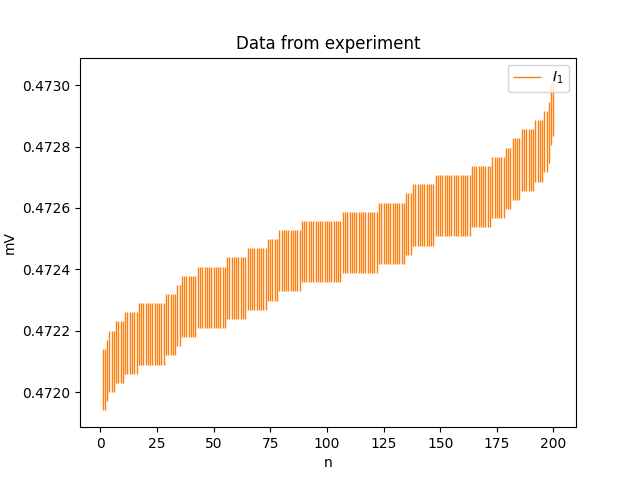
\includegraphics[width=15cm]{pics/input.png}
    \caption{График входных интервальных данных}
    \label{fig:input}
\end{figure}

\begin{figure}[H]
    \centering
    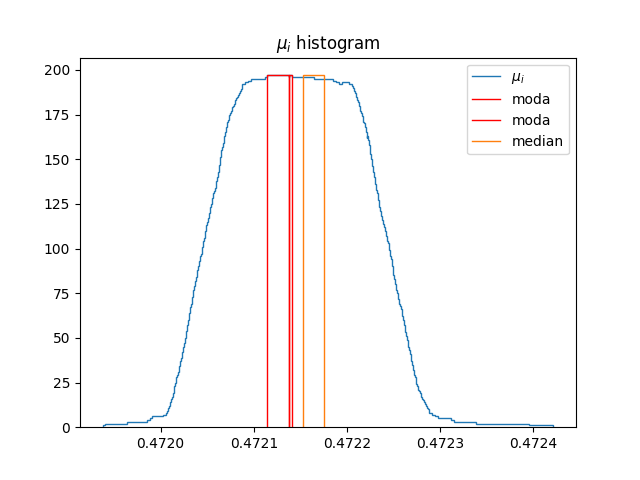
\includegraphics[width=12cm]{pics/mu_hist.png}
    \caption{Гистограмма частот $\mu_i$ для интервалов $z_i$}
    \label{fig:mu_hist}
\end{figure}

\begin{figure}[H]
    \centering
    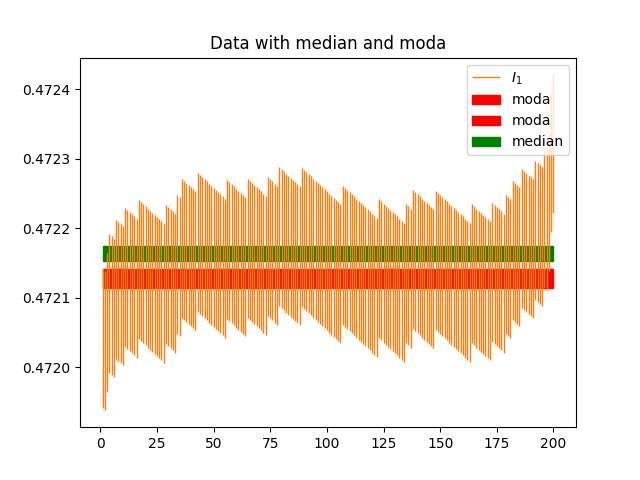
\includegraphics[width=12cm]{pics/data_med_mod.png}
    \caption{График входных данных с изображенными на нём медианой и модой}
    \label{fig:med_mod}
\end{figure}

\subsection{Числовые значения}
$$JK(x) = -0.1730642550574791$$
$$med(x) = [0.47215261724, 0.47217476034]$$
$$mod(x) = [0.4721145618, 0.47213771724] \cup [0.47213819628, 0.47214079999999997]$$

\section{Обсуждение}
\begin{enumerate}
    \item Исходя из значения коэффициента Жаккара можно сказать, что данные не являются совсместными.
    \item Интервалы медианы и моды несовместны.
    \item Различие в положениях медианы и моды при этом не велико, что хорошо объясняется графиком \ref{fig:mu_hist}, демонстрирующим унимодальность распределения.
\end{enumerate}
\end{document}
